\chapter{Dasar Telematika}

\section{Tujuan}
\begin{enumerate}
    \item Belajar menyusun dan menganalisa rangkaian
    \item Mengetahui fungsi setiap komponen dan cara implementasinya
    \item Untuk memperkenalkan beberapa konsep dasar dan teknik laboratorium dalam bekerja menggunakan peralatan elektronika dan soldering
\end{enumerate}

\section{Dasar Teori}
Seven Segment Display memiliki 7 Segmen dimana setiap segmen dikendalikan secara ON dan OFF untuk menampilkan angka yang diinginkan. 
Angka-angka dari 0 (nol) sampai 9 (Sembilan) dapat ditampilkan dengan menggunakan beberapa kombinasi Segmen. Selain 0 – 9, Seven Segment 
Display juga dapat menampilkan Huruf Hexadecimal dari A sampai F. Segmen atau elemen-elemen pada Seven Segment Display diatur menjadi 
bentuk angka “8” yang agak miring ke kanan dengan tujuan untuk mempermudah pembacaannya. Pada beberapa jenis Seven Segment Display, 
terdapat juga penambahan “titik” yang menunjukan angka koma decimal.  Terdapat beberapa jenis Seven Segment Display, diantaranya adalah 
Incandescent bulbs, fluorescent lamps (FL), Liquid Crystal Display (LCD) dan Light Emitting Diode (LED).

Salah satu jenis Seven Segment Display yang sering digunakan adalah 7 Segmen yang menggunakan LED (Light Emitting Diode) sebagai penerangnya.  
LED 7 Segmen ini umumnya memiliki 7 Segmen atau elemen garis dan 1 segmen titik yang menandakan “koma” Desimal. Jadi Jumlah keseluruhan segmen 
atau elemen LED sebenarnya adalah 8. Cara kerjanya pun boleh dikatakan mudah, ketika segmen atau elemen tertentu diberikan arus listrik, maka 
Display akan menampilkan angka atau digit yang diinginkan sesuai dengan kombinasi yang diberikan.

Logam yang biasa digunakan adalah timah yang memiliki titik leleh antara 90 hingga 450 \degree C. Timah dapat dilelehkan menggunakan solder yang dipanaskan. 
Ketika lelehan timah ini mendingin dan mengeras akan membentuk saluran yang dapat dilalui oleh listrik.  Soldering biasa dilakukan pada PCB (Printed Circuit Board) 
dimana pada PCB terdapat lubang-lubang kecil dimana kaki komponen dapat dimasukan kemudian kaki komponen dapat disolder untung memasang komponen tersebut.

Teknik soldering merupakan proses penggabungan dua komponen logam dengan menggunakan timah solder yang dicairkan untuk membentuk sambungan yang konduktif. 
Proses ini umumnya digunakan dalam industri elektronik untuk menghubungkan komponen pada papan sirkuit. Dalam keadaan di mana sambungan perlu diperbaiki 
atau komponen diganti, teknik desoldering diterapkan. Desoldering adalah proses penghapusan solder dari suatu sambungan untuk melepaskan komponen dari papan sirkuit. 
Kedua teknik ini memerlukan alat khusus, presisi, dan keahlian untuk memastikan sambungan yang efektif dan untuk mencegah kerusakan pada papan atau komponen.


\section{Tugas Pendahuluan}
\begin{enumerate}
    \item Jelaskan bagaimana cara kontrol 7-segment anoda dan katoda?
    \item Buat schematic untuk menampilkan nomor kelompok menggunakan dua 7-segment!
\end{enumerate}

\section{Alat dan Komponen}
\subsection{Alat}
\begin{enumerate}
    \item Soldering kit
    \item Timah 0.8 mm
    \item Power source
    \item Sikat 
    \item IPA (Isopropyl alcohol)
    \item Flux
    \item Solder Pasta
\end{enumerate}

\subsection{Komponen}
\begin{enumerate}
    \item PCB 4x6 cm                        (1x)
    \item Header Female                     (1x)
    \item Resistor 330-ohm 			        (1x)
    \item White Housing 2 Pin			    (1x)
    \item 7-Segment 0.56-inch Common Katoda	(2x)
    \item Modul LED Chaser kit              (1x)
\end{enumerate}
\section{Eksperimen 1: Teknik Desoldering}
\begin{enumerate}
    \item Dokumentasikan pcb yang akan di desolder.
    \item Siapkan semua peralatan yang disebutkan dan panaskan solder terlebih dahulu
        \begin{figure}[H]
            \centering
            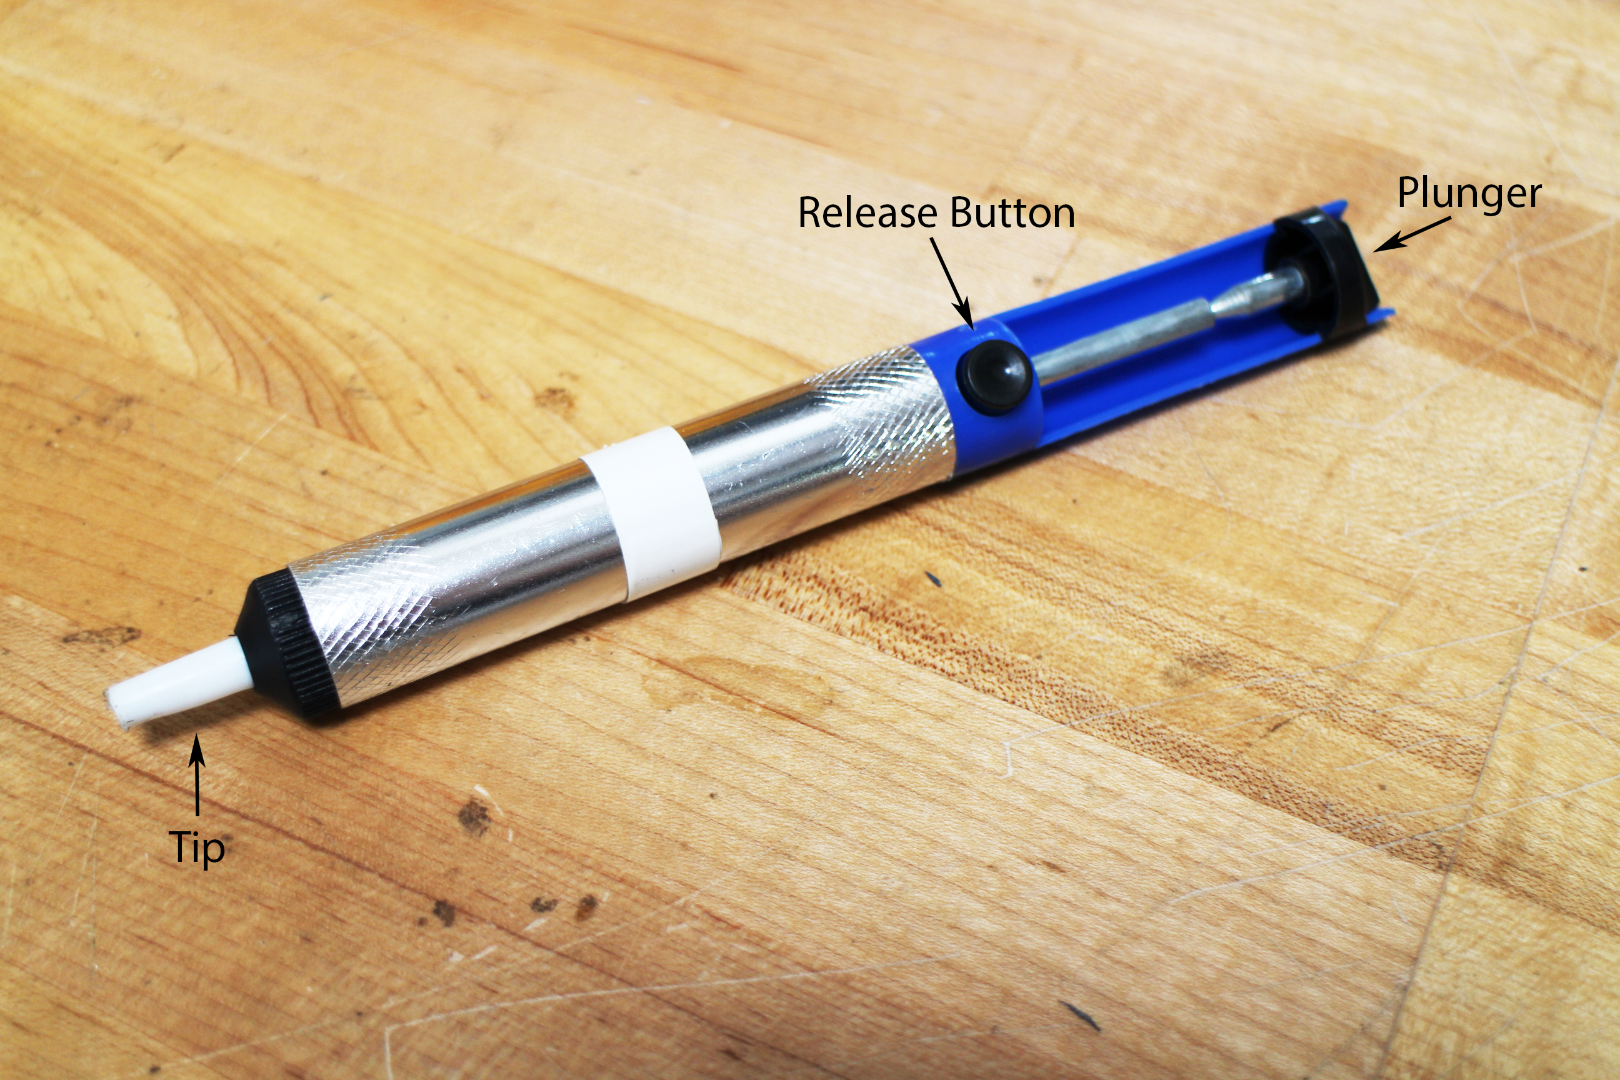
\includegraphics[width=0.6\linewidth]{P2/img/desolder.png}
            \caption{Desolder}
            \label{fig:desolder}
        \end{figure}
    \item Panaskan timah yang ingin  dilepaskan dengan besi solder
    \item Tekan plunger.
    \item Setelah timah menjadi cair, letakkan ujung pompa desolder tepat pada timah yang ingin dilepaskan.
    \item Lepaskan plunger dengan menekan penahan (release button).
    \item Lepaskan komponen yang bebas.
    \item Ulangi langkah 2-6 untuk menghilangkan timah berlebih.
    \item Buang timah di dalam pompa dengan terus menekan dan melepaskan plunger.
    \item Amati output yang dihasilkan, dokumentasikan hasil output dalam bentuk lampiran
\end{enumerate}
\section{Eksperimen 2: Teknik Soldering}
\begin{figure}[H]
    \centering
    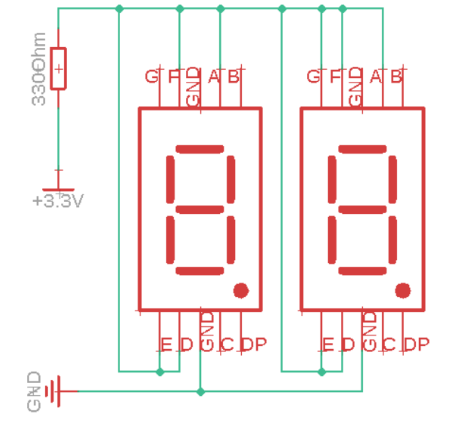
\includegraphics[width=0.4\linewidth]{P2/img/schematics.png}
    \caption{Schematics 7-Segment}
    \label{fig:schematics7Segment}
\end{figure}

\begin{figure}[H]
    \centering
    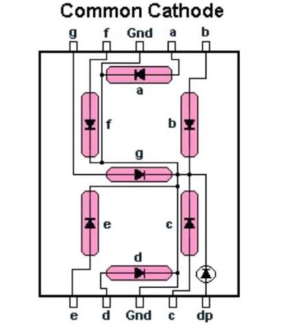
\includegraphics[width=0.4\linewidth]{P2/img/7segment.png}
    \caption{Pin Referensi 7-Segment Katoda}
    \label{fig:Referensi7Segment}
\end{figure}
\begin{enumerate}
    \item Siapkan semua peralatan yang disebutkan dan panaskan solder terlebih dahulu
    \item Pasang header untuk 7-segment pada PCB lalu disolder menggunakan timah. (Pastikan Header terpasang dengan jarak yang sesuai dengan panjang 7-segment).
    \item Kaki-kaki dari komponen  elektronik yang terpasang di pcb dihadapkan ke atas, dan jika kaki-kaki tersebut panjang maka bisa dibengkokkan sehingga saat hendak disolder komponen tersebut tidak rentan bergoyang yang nantinya menyusahkan proses menyolder
    \item Tambahkan pasta fluks pada area copper pad secukupnya, untuk instruksi menyolder bisa diperhatikan di gambar berikut
        \begin{figure}[H]
            \centering
            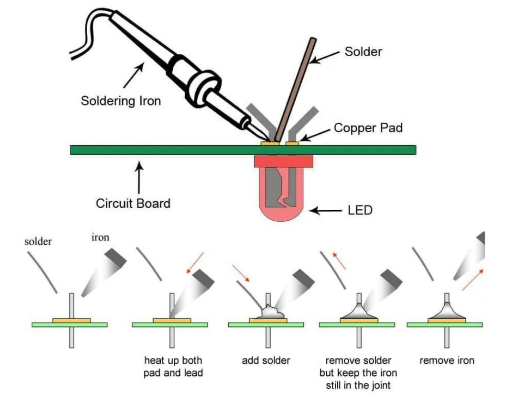
\includegraphics[width=0.6\linewidth]{P2/img/solder1.png}
            \caption{Prosedur Soldering (1)}
            \label{fig:ProsedurSoldering1}
        \end{figure}
        \begin{figure}[H]
            \centering
            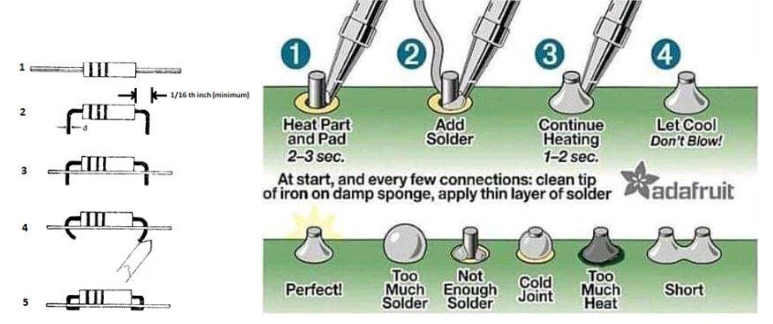
\includegraphics[width=0.8\linewidth]{P2/img/solder2.png}
            \caption{Prosedur Soldering (2)}
            \label{fig:ProsedurSoldering2}
        \end{figure}
    \item Letakkan soldering iron ke permukaan copper pad dan kaki dari komponen yang hendak disolder sehingga panasnya menyebar. Agar panas dari soldering iron lebih cepat menyebar ke copper pad dan kaki komponen, tambahkan sedikit timah ke bagian soldering iron 
    yang nantinya berkontak sehingga luas permukaan penghantar panas bertambah dan proses menyolder menjadi relatif lebih mudah
    \item Setelah copper pad dan kaki komponen dirasa cukup panas, tambahkan timah solder ke arah tersebut hingga timah meleleh dan terbentuk seperti cone kerucut seperti di peraga, lalu angkat timah solder dan soldering iron secara berturut-turut
    \item Gunakan modul 7-segment dan hubungkan rangkaian menggunakan timah yang dipanaskan dengan solder sesuai schematic diatas, lakukanlah proses menyolder ini ke semua komponen elektronik yang diperlukan
    \item Di akhir proses meyolder, seringkali terdapat bekas pasta fluks yang membuat pcb terlihat kurang bersih, untuk membersihkannya gunakan sikat gigi yang dibasahi atau dicelupkan ke IPA dan gosokkan secara searah ke pcb yang dirasa kotor oleh sisa pasta fluks hingga dirasa cukup bersih
    \item Setelah semua komponen terhubung sesuai intruksi, nyalakan power source untuk mencoba rangkaian. Sebelumnya Periksa hasil solder dengan multimeter untuk mengecek konektivitas antar sambungan
    \item Amati output yang dihasilkan, dokumentasikan hasil output dalam bentuk lampiran
        \\ Contoh hasil
        \begin{figure}[H]
            \centering
            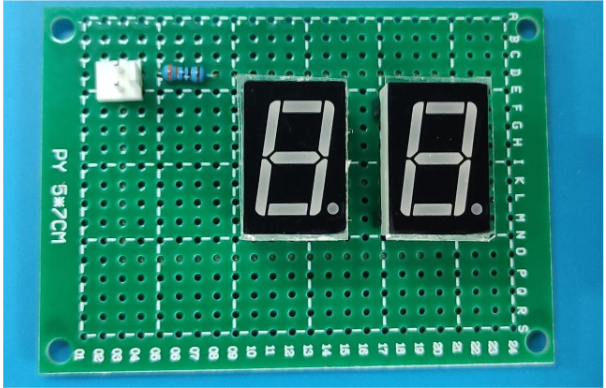
\includegraphics[width=0.8\linewidth]{P2/img/contohhasil1.png}
            \caption{Hasil Soldering Tampak Depan}
            \label{fig:HasilTampakDepan}
        \end{figure}
        \begin{figure}[H]
            \centering
            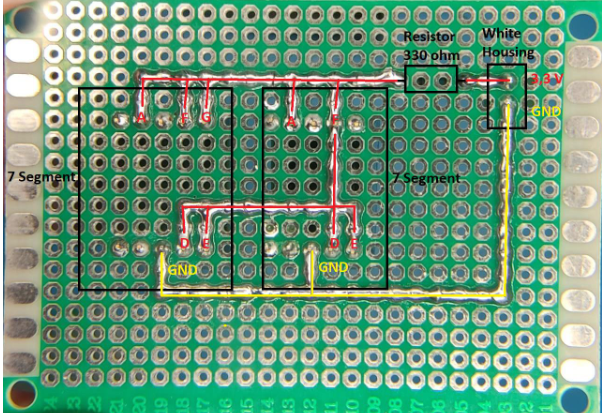
\includegraphics[width=0.8\linewidth]{P2/img/contohhasil2.png}
            \caption{Hasil Soldering Tampak Belakang}
            \label{fig:HasilTampakBelakang}
        \end{figure}
\end{enumerate}

\section{Eksperimen 3: Teknik Soldering Uap}
\subsection{Percobaan 1: Penyolderan SMD}
\begin{enumerate}
    \item Siapkan semua peralatan dan komponen yang dibutuhkan.
    \item Siapkan PCB yang akan disolder
    \item Tuangkan solder pasti di tempat komponen yang akan disolder.
    \item Jika solder pasta sudah tertuang di semua tempat komponen. Lanjutkan memasang komponen pada posisinya sesuai dengan tabel dibawah ini.
    
    \item Jika komponen sudah terpasang, panaskan solder uap dan tunggu hingga panas (+-400$^{\circ}$C).
    \item Solder dengan cara dekatkan ujung solder uap ke komponen yang akan di sambungkan. Pastikan sudah melekat ketika akan berpindah ke komponen lain.
    \item Solder komponen through hole (LED, Potensio, Pin Header) dengan timah.
    \item Hubungkan PCB dengan power supply.
    \item Amati output yang dihasilkan, dokumentasikan hasil output dalam bentuk lampiran
\end{enumerate}


\begin{center}
	\colorbox{pink}{\parbox{0.8\linewidth}{\textbf{Tips:} Ketika menyolder SMD, disarankan dimulai dari yang paling rumit terdahulu (IC),
    setelah itu resistor/kapasitor. Penyolderan komponen through-hole dapat dilakukan
    setelah komponen SMD tersolder semua.}}
\end{center}

\subsection{Percobaan 2: Mengatur Kecepatan LED Chaser}
\begin{enumerate}
    \item Beri daya pada modul LED Chaser
    \item Putar VAR-RES searah jarum jam, amati apa yang terjadi
    \item Putar VAR-RES berlawanan jarum jam, amati apa yang terjadi
    \item Amati output yang dihasilkan, dokumentasikan hasil output dalam bentuk lampiran
\end{enumerate}

\begin{figure}[H]
    \centering
    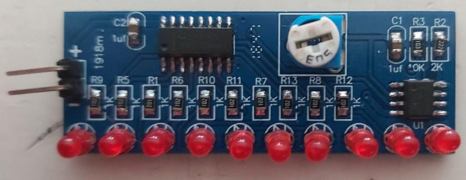
\includegraphics[width=0.8\linewidth]{P2/img/HasilSMD.png}
    \caption{Hasil SMD}
    \label{fig:HasilSMD}
\end{figure}